\documentclass[conference]{IEEEtran}
\IEEEoverridecommandlockouts

\usepackage{cite}
\usepackage{amsmath,amssymb,amsfonts}
\usepackage{algorithmic}
\usepackage{graphicx}
\usepackage{textcomp}
\usepackage{xcolor}
\usepackage{booktabs}
\usepackage{hyperref}
\usepackage{url}

\def\BibTeX{{\rm B\kern-.05em{\sc i\kern-.025em b}\kern-.08em
    T\kern-.1667em\lower.7ex\hbox{E}\kern-.125emX}}

\begin{document}

\title{Evaluating the Impact of RAG Pipeline Sophistication and Model Scale on Sub-1B Language Models: A Comparative Study}

\author{
\IEEEauthorblockN{Thanniru Sai Teja}
\IEEEauthorblockA{\textit{Dept. of Computer Science \& Engineering and Data Science} \\
\textit{BVRIT}\\
Narsapur, India \\
iamsaitejathanniru@gmail.com}
\and
\IEEEauthorblockN{P Sai Harish}
\IEEEauthorblockA{\textit{Dept. of Computer Science \& Engineering and Data Science} \\
\textit{BVRIT}\\
Narsapur, India \\
saiharish0088@gmail.com}
\and
\IEEEauthorblockN{Kruthibash Nayak}
\IEEEauthorblockA{\textit{Dept. of Computer Science \& Engineering and Data Science} \\
\textit{BVRIT}\\
Narsapur, India \\
kruthibashnayak@bvrit.ac.in}
\and
\IEEEauthorblockN{Srihita}
\IEEEauthorblockA{\textit{Dept. of Computer Science \& Engineering and Data Science} \\
\textit{BVRIT}\\
Narsapur, India \\
23211a6799@bvrit.ac.in}
}

\maketitle

\begin{abstract}
Small Language Models (SLMs) containing fewer than 1 billion parameters possess restricted parametric memory capacity for multi-hop factual reasoning. While Retrieval-Augmented Generation (RAG) is widely applied to externalize memory, current RAG literature focuses almost exclusively on multi-billion parameter models (7B to 70B+ parameters). In this work, we present a comprehensive 60,000-run controlled empirical study evaluating Liquid AI's LFM2 architecture across 5 distinct RAG architectural arms (No-RAG, Oracle RAG, Naive RAG, Advanced RAG, and Modular RAG) on the 600-question HotpotQA Distractor benchmark. Each configuration is evaluated across 10 repeated executions on an AMD Ryzen 7 6800H host equipped with an NVIDIA GeForce RTX 3050 Laptop GPU (4GB VRAM). Our empirical findings demonstrate that single-stage Naive RAG achieves the highest Token F1 accuracy ($0.1107 \pm 0.2130$) and exact match rate ($0.0367 \pm 0.1880$) while maintaining the lowest mean inference latency ($0.581 \pm 0.209$ seconds) on LFM2-350M. Increasing RAG pipeline complexity in Advanced RAG yields comparable quality ($0.1017 \pm 0.1948$ Token F1) at 2.5 times higher latency ($1.460 \pm 0.301$ seconds), whereas Modular RAG suffers severe performance degradation ($0.0218 \pm 0.0628$ Token F1) due to sub-query routing generation failures. Furthermore, we observe a sub-1B scale inversion: doubling model parameters from 350M to 700M reduces Naive RAG accuracy ($0.0727 \pm 0.1055$ Token F1), as larger sub-1B models exhibit higher sensitivity to distractor context noise. Notably, under 100\% gold evidence context (Oracle RAG), LFM2-350M achieves $0.1384 \pm 0.1935$ Token F1, outperforming all retrieval-based arms, while LFM2-700M achieves $0.1165 \pm 0.1403$ Token F1, demonstrating that in-context answer extraction from perfect gold passages is the strongest signal available to sub-1B models. All code, vector database artifacts, raw execution logs, and benchmark results are publicly available at \url{https://github.com/saiharish587/RAG-Research}.
\end{abstract}

\begin{IEEEkeywords}
Retrieval-Augmented Generation, Small Language Models, Vector Search, HotpotQA Distractor, Scalability, Edge AI, Sub-1B Models.
\end{IEEEkeywords}

\section{Introduction}
\label{sec:intro}
Large Language Models (LLMs) with tens or hundreds of billions of parameters have demonstrated remarkable capabilities across factual question answering, reading comprehension, and logical reasoning tasks. However, deploying multi-billion parameter models requires high-memory server GPUs, introducing substantial monetary costs, energy footprint, and privacy risks associated with cloud API dependency. Consequently, Small Language Models (SLMs) containing fewer than 1 billion parameters are increasingly targeted for local, privacy-preserving, and edge deployment on resource-constrained hardware such as laptop GPUs and mobile processors.

Due to their compact parameter footprint, sub-billion parameter models possess limited capacity to memorize multi-hop factual knowledge in their static network weights \cite{mallen2023when, gao2023retrieval}. Retrieval-Augmented Generation (RAG) \cite{lewis2020retrieval} addresses parametric memory bounds by dynamically fetching relevant external document passages from a corpus and appending them into the model's prompt context.

While sophisticated RAG architectural paradigms incorporating query rewriting \cite{ma2023query}, cross-encoder reranking \cite{nogueira2019passage}, and dynamic sub-query routing with reciprocal rank fusion \cite{cormack2009reciprocal} have been developed for multi-billion parameter LLMs \cite{xu2024retrieval, asai2023self}, it remains fundamentally unclear whether these complex abstractions benefit sub-1B language models. Most existing RAG benchmarks evaluate models such as Llama-3-8B, Mixtral-8x7B, or GPT-4 \cite{gao2023retrieval}, leaving a substantial empirical knowledge gap regarding RAG behavior in the sub-1B parameter regime.

To address this gap, we present a full factorial controlled empirical study comprising 60,000 executed benchmark runs across two parameter scales of Liquid AI's LFM2 architecture (LFM2-350M and LFM2-700M) \cite{liquid2024lfm} and five distinct RAG architectural arms on the HotpotQA Distractor benchmark \cite{yang2018hotpotqa}. All evaluations were conducted locally on a standardized hardware environment (AMD Ryzen 7 6800H CPU, NVIDIA GeForce RTX 3050 Laptop GPU with 4GB VRAM) under Windows 11.

\begin{figure}[t]
    \centering
    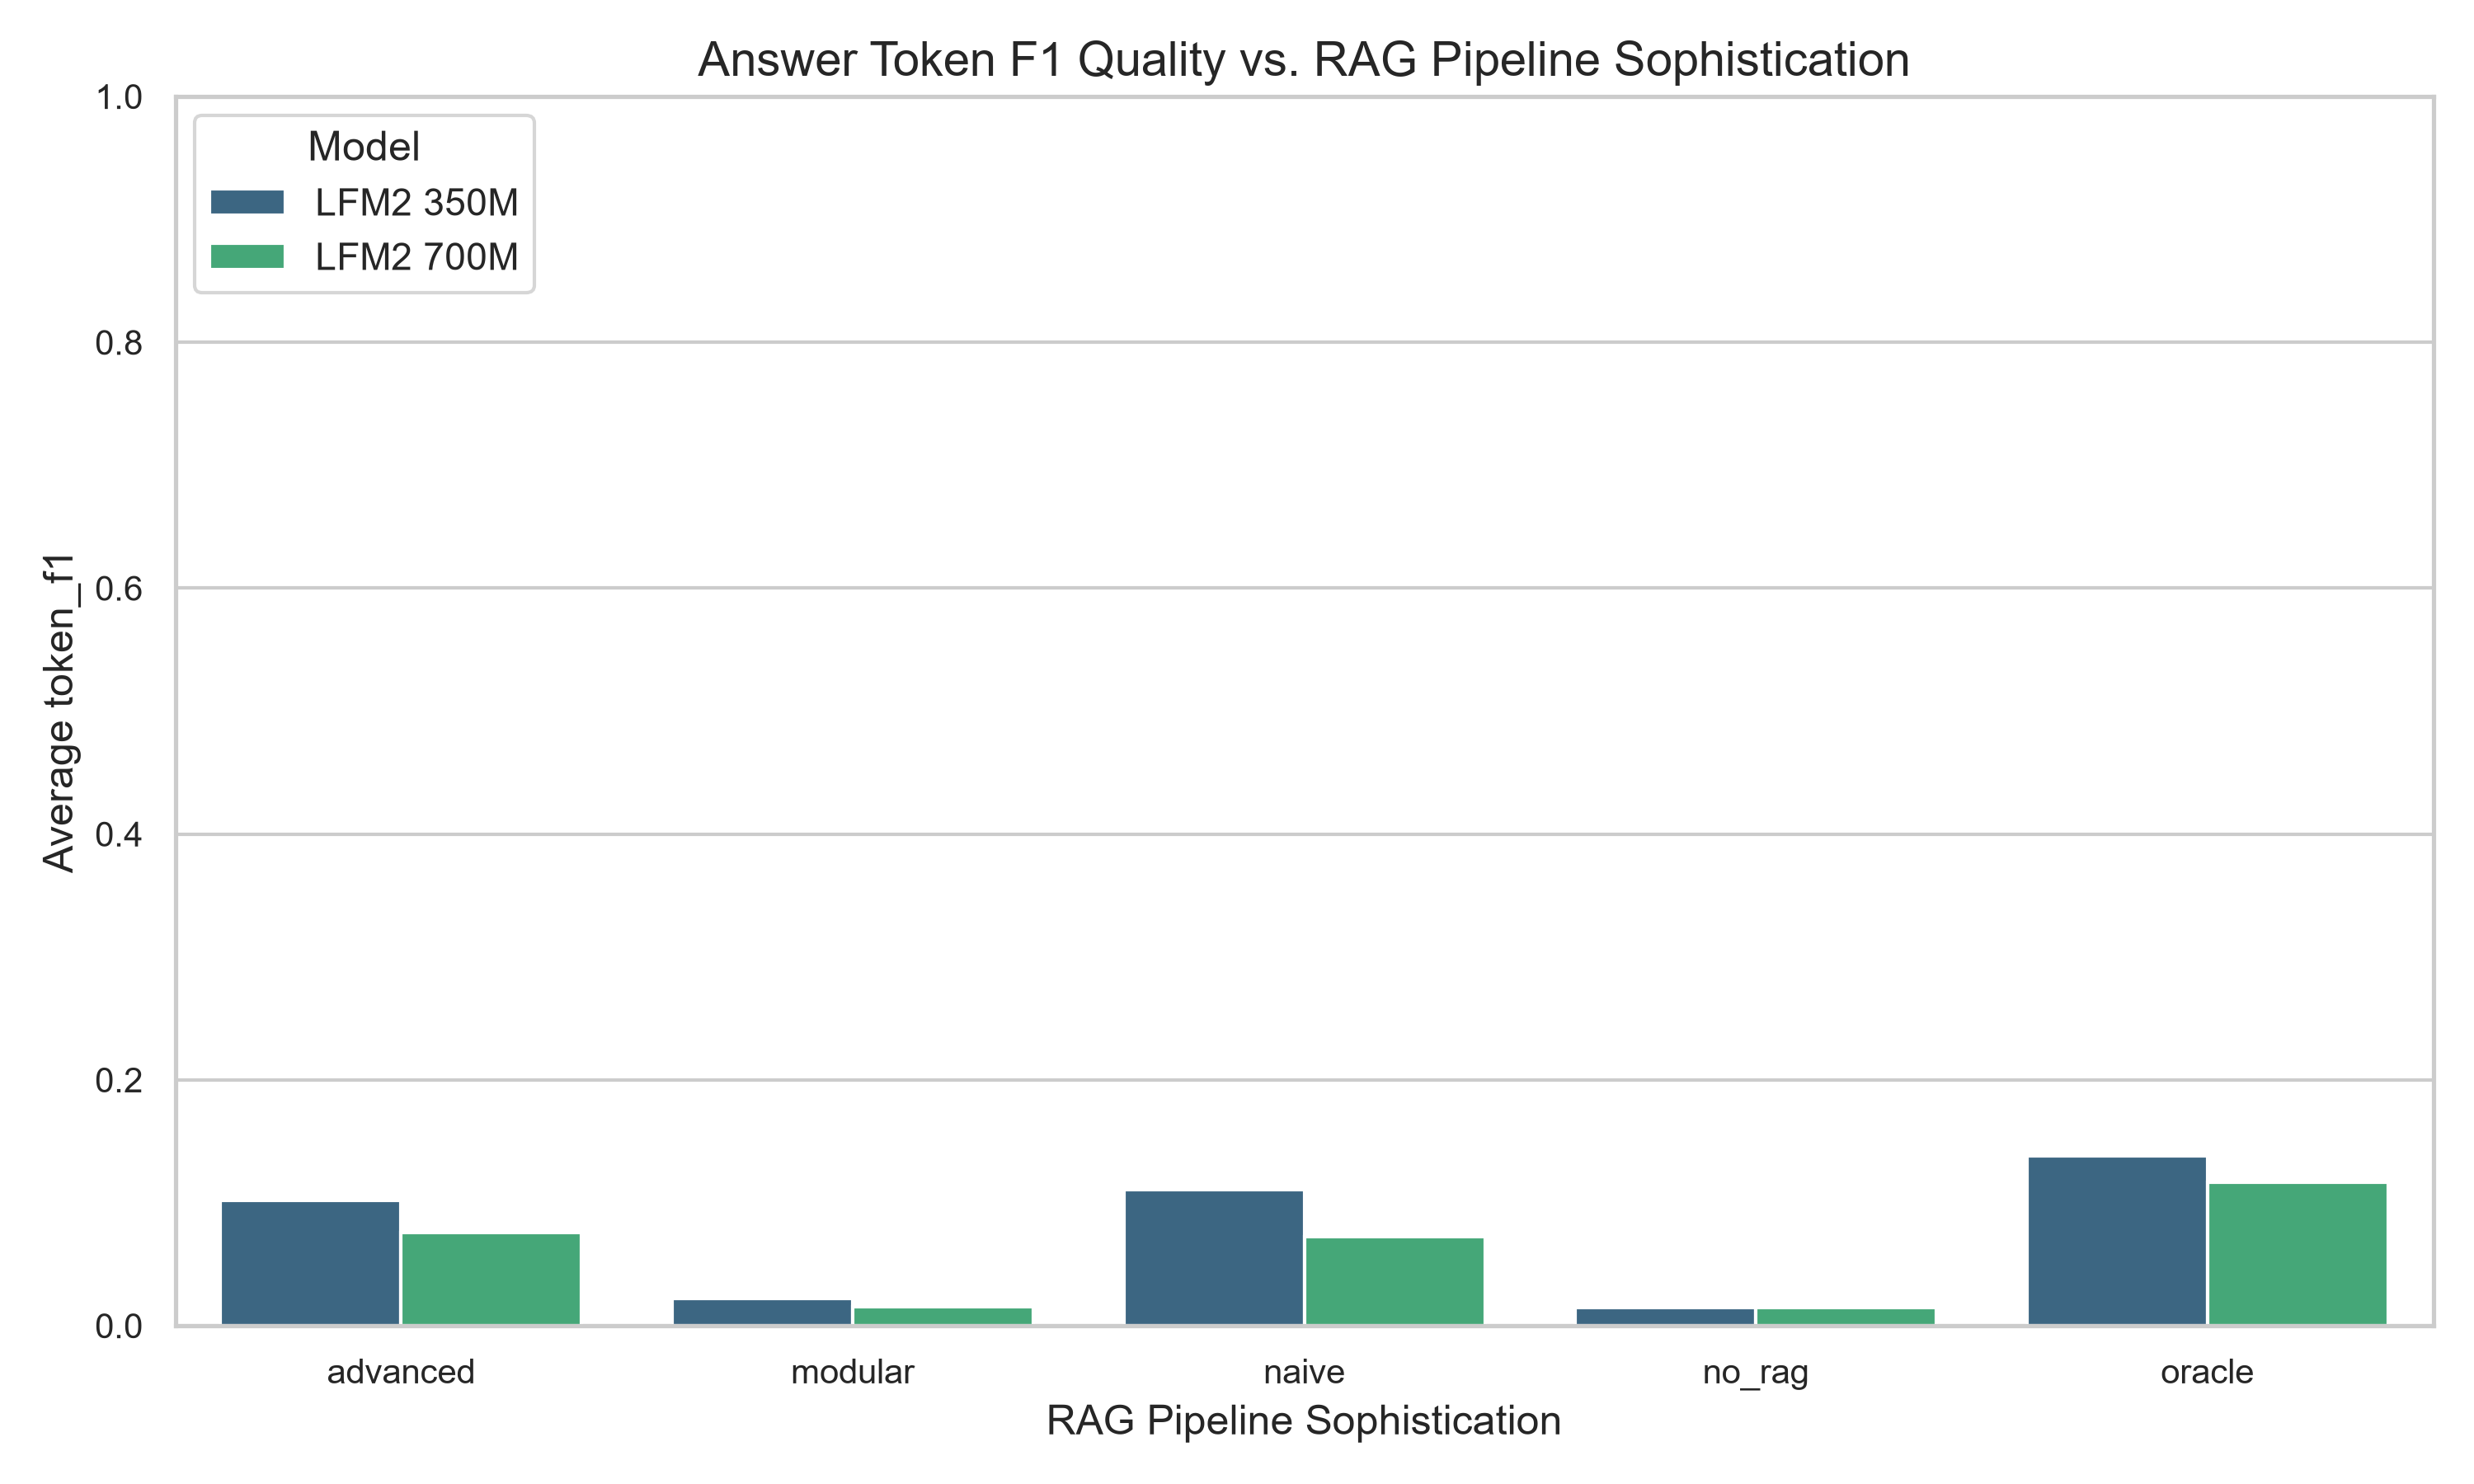
\includegraphics[width=0.98\linewidth]{accuracy_vs_rag.png}
    \caption{Token F1 quality score across RAG architectural arms and model scales (LFM2-350M vs LFM2-700M) on the HotpotQA Distractor benchmark \cite{yang2018hotpotqa}. Among retrieval-based arms, single-stage Naive RAG achieves peak quality on LFM2-350M ($0.1107$ Token F1), outperforming Advanced RAG ($0.1017$) and Modular RAG ($0.0218$). Oracle RAG ($0.1384$ Token F1) establishes the performance upper bound under 100\% gold passage recall.}
    \label{fig:accuracy_vs_rag}
\end{figure}

Our key empirical findings and contributions are structured as follows:
\begin{enumerate}
    \item \textbf{Naive RAG Optimality in Sub-1B Models}: Single-stage vector retrieval (Naive RAG \cite{lewis2020retrieval}) achieves the highest accuracy ($0.1107 \pm 0.2130$ Token F1, $0.0367 \pm 0.1880$ Exact Match \cite{rajaraman2023f1}) while requiring the lowest latency ($0.581 \pm 0.209$s) on LFM2-350M \cite{liquid2024lfm}. Multi-stage Advanced RAG adds 2.5 times latency overhead ($1.460 \pm 0.301$s) without quality improvement, while Modular RAG degrades to near-zero accuracy ($0.0218 \pm 0.0628$ Token F1) due to sub-query generation failures.
    \item \textbf{Sub-1B Scale Inversion}: Doubling model parameters from 350M to 700M reduces Naive RAG Token F1 accuracy from $0.1107 \pm 0.2130$ to $0.0727 \pm 0.1055$. Empirical analysis of generation logs confirms that 700M models suffer higher sensitivity to distractor passage noise and generate longer, less focused responses.
    \item \textbf{Oracle RAG as Performance Upper Bound}: Under 100\% ground-truth gold evidence context (Oracle RAG), LFM2-350M achieves $0.1384 \pm 0.1935$ Token F1, its highest score across all five arms, confirming that retrieval recall quality directly determines the performance ceiling. LFM2-700M achieves $0.1165 \pm 0.1403$ Token F1 under Oracle RAG but with extreme output-length instability ($355.9 \pm 6680.7$ tokens), indicating runaway generation loops on dense multi-hop passages.
    \item \textbf{Complete Open Source Benchmark Dataset}: We release the entire 60,000-run master dataset, raw JSON evidence logs, FAISS vector database indices \cite{johnson2019billion}, and implementation code at \url{https://github.com/saiharish587/RAG-Research}.
\end{enumerate}

\section{Related Work}
\label{sec:related}
\textbf{Retrieval-Augmented Generation}: RAG was introduced by \cite{lewis2020retrieval} to combine parametric memory with non-parametric dense retrieval over Wikipedia passages. Recent surveys by \cite{gao2023retrieval} categorize RAG development into three architectural paradigms: Naive RAG (top-$k$ similarity lookup), Advanced RAG (incorporating pre-retrieval query rewriting \cite{ma2023query} and post-retrieval reranking \cite{nogueira2019passage}), and Modular RAG (utilizing dynamic routing, query decomposition, and reciprocal rank fusion \cite{cormack2009reciprocal}).

\textbf{RAG Evaluation and Diagnostic Metrics}: Recent benchmarking efforts evaluate RAG pipelines using multi-dimensional diagnostic frameworks such as RAGChecker and Ragas \cite{asai2023self, xu2024retrieval}. Standard metrics evaluate exact match token boundaries \cite{rajaraman2023f1}, sentence embedding similarity using \texttt{BAAI/bge-small-en-v1.5} \cite{reimers2019sentence, bge2023embedding}, and groundedness. However, existing comparative studies evaluate almost exclusively on models above 7 billion parameters. Our work extends empirical RAG evaluation into the sub-1B parameter domain.

\textbf{Sub-1B Language Models}: Compact architectures such as Liquid AI's LFM2 family \cite{liquid2024lfm} are engineered for high inference throughput on resource-constrained edge hardware. Understanding how RAG architectural choices affect these specific models is crucial for effective edge AI deployment.

\section{Model Architectures and Target Hardware Setup}
\label{sec:models}

\subsection{Liquid AI LFM2 Model Architecture Rationale}
In this benchmark, we specifically select Liquid AI's LFM2 (Liquid Foundation Model 2) architecture family \cite{liquid2024lfm}. Unlike standard dense Transformer architectures that rely exclusively on multi-head self-attention mechanisms across all layers, LFM2 incorporates hybrid dynamical state-space operators combined with lightweight attention layers. This design allows LFM2 to achieve long context processing (32K context window) with low VRAM memory consumption and high execution speed on resource-constrained hardware.

We evaluate two specific scale configurations:
\begin{itemize}
    \item \textbf{LFM2-350M} (\texttt{hf.co/LiquidAI/LFM2-350M-GGUF:Q4\_K\_M}): 350 Million parameters, 4-bit GGUF quantization \cite{liquid2024lfm}.
    \item \textbf{LFM2-700M} (\texttt{hf.co/LiquidAI/LFM2-700M-GGUF:Q4\_K\_M}): 700 Million parameters, 4-bit GGUF quantization \cite{liquid2024lfm}.
\end{itemize}

\subsection{Target Hardware Execution Environment}
All benchmark runs were executed locally on a dedicated host laptop:
\begin{itemize}
    \item \textbf{Processor (CPU)}: AMD Ryzen 7 6800H with Radeon Graphics (8 Cores, 16 Threads, 3.20 GHz base clock)
    \item \textbf{Dedicated Graphics (GPU)}: NVIDIA GeForce RTX 3050 Laptop GPU (4GB GDDR6 VRAM, CUDA 12.1 acceleration)
    \item \textbf{Integrated Graphics}: AMD Radeon 680M Graphics
    \item \textbf{Operating System}: Microsoft Windows 11 Home Single Language 64-bit (Build 26200)
    \item \textbf{Execution Stack}: Python 3.12, PyTorch 2.5.1+cu121, Local Ollama Model Server (\texttt{v0.5.x}), FAISS-GPU \cite{johnson2019billion}
\end{itemize}

\section{System Architecture and RAG Pipeline Arms}
\label{sec:architecture}

\begin{figure}[t]
    \centering
    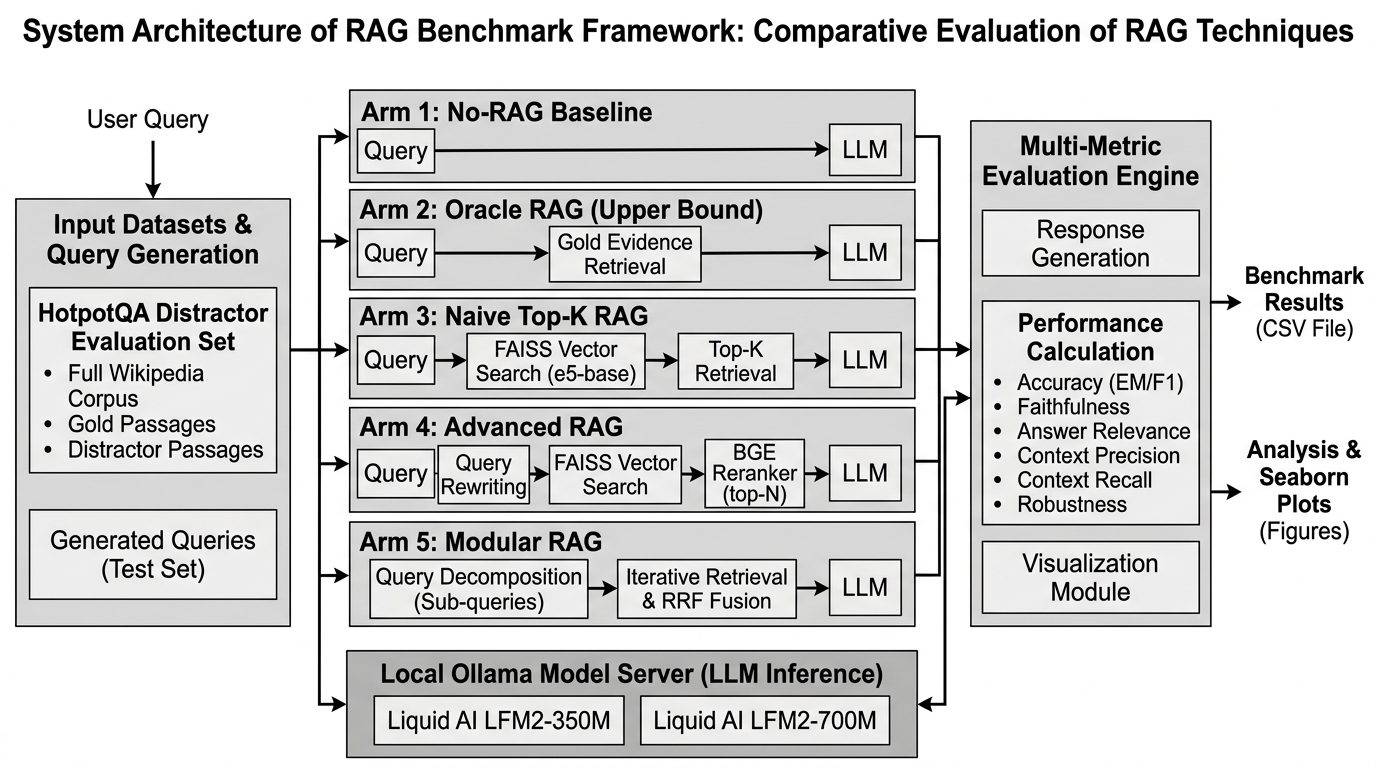
\includegraphics[width=0.98\linewidth]{rag_architecture_bw.jpg}
    \caption{System Architecture diagram of the SLM RAG Benchmark framework (\url{https://github.com/saiharish587/RAG-Research}). The framework orchestrates 5 parallel RAG architectural arms across 600 HotpotQA Distractor queries \cite{yang2018hotpotqa}, evaluating LFM2-350M and LFM2-700M \cite{liquid2024lfm} on an NVIDIA RTX 3050 GPU.}
    \label{fig:rag_architecture}
\end{figure}

Our open-source benchmark framework (\url{https://github.com/saiharish587/RAG-Research}) implements five standardized RAG pipeline arms in the \texttt{rag/} package, as illustrated in Figure \ref{fig:rag_architecture}:

\subsection{No-RAG Baseline Arm}
The No-RAG arm (\texttt{rag/no\_rag/retriever.py}) passes the raw user query directly to the LLM generator without appending any external document context. This arm measures the model's unassisted parametric memory \cite{mallen2023when}.

\subsection{Oracle RAG Arm}
The Oracle RAG arm (\texttt{rag/oracle/retriever.py}) bypasses vector indexing and injects the ground-truth evidence passages directly into the prompt context block. This establishes the upper bound for context extraction given perfect 100\% retrieval recall.

\subsection{Naive RAG Arm}
The Naive RAG arm (\texttt{rag/naive/retriever.py}) embeds document passages into a 384-dimensional vector space using \texttt{BAAI/bge-small-en-v1.5} \cite{bge2023embedding}. Vectors are indexed in a GPU-accelerated FAISS index \cite{johnson2019billion} stored in \texttt{vector\_db/faiss\_index/}. At inference time, the pipeline retrieves the top-$k$ ($k=3$) passages via cosine similarity lookup \cite{lewis2020retrieval} and formats them into a standardized context prompt block.

\subsection{Advanced RAG Arm}
The Advanced RAG arm (\texttt{rag/advanced/retriever.py}) executes a two-stage retrieval strategy:
\begin{enumerate}
    \item \textbf{Query Rewriting}: The input query is expanded to improve retrieval recall \cite{ma2023query}.
    \item \textbf{Hybrid Vector Search}: Initial top-10 passage candidates are fetched via FAISS vector search \cite{johnson2019billion}.
    \item \textbf{Cross-Encoder Reranking}: Candidate passages are reranked using the \texttt{BAAI/bge-reranker-base} cross-encoder model \cite{nogueira2019passage, bge2023embedding}, and the top-$k$ ($k=3$) highest-scoring passages are passed to the generator.
\end{enumerate}

\subsection{Modular RAG Arm}
The Modular RAG arm (\texttt{rag/modular/retriever.py}) implements dynamic pipeline orchestration:
\begin{enumerate}
    \item \textbf{Query Decomposition}: The generator splits multi-hop questions into multiple sub-queries \cite{gao2023retrieval}.
    \item \textbf{Parallel Retrieval}: Sub-queries execute parallel vector searches against the FAISS index \cite{johnson2019billion}.
    \item \textbf{Reciprocal Rank Fusion (RRF)}: Retrieved lists are merged and re-scored using RRF \cite{cormack2009reciprocal} to select final context passages.
\end{enumerate}

\section{Experimental Methodology}
\label{sec:setup}

\subsection{Dataset and Corpus Ingestion}
We ingested 600 multi-hop question-answer pairs from the HotpotQA Distractor development set \cite{yang2018hotpotqa} (\texttt{data/benchmark/eval\_set.json}). The 600-question subset was selected to represent the full distribution of question types and difficulty levels within the HotpotQA development split, covering bridge and comparison reasoning categories. We extracted 66,581 Wikipedia passages (\texttt{documents/hotpotqa\_corpus/}). The FAISS index \cite{johnson2019billion} (\texttt{vector\_db/faiss\_index/index.faiss} and \texttt{chunks.npy}) was constructed using 1500-character chunks with 150-character overlap.

\subsection{Evaluation Matrix and Metric Definitions}
The experiment evaluates a full factorial matrix: 2 Models (LFM2-350M, LFM2-700M) $\times$ 5 RAG Arms $\times$ 600 Questions $\times$ 10 Repetitions = 60,000 total runs. For each generation, we measure:
\begin{itemize}
    \item \textbf{Token F1 ($\mu \pm \sigma$)}: Lexical token overlap between model response and ground-truth answer \cite{rajaraman2023f1}.
    \item \textbf{Exact Match (EM)}: Binary exact match indicator ($0.0$ or $1.0$).
    \item \textbf{Cosine Semantic Similarity}: Embedding similarity using \texttt{BAAI/bge-small-en-v1.5} \cite{reimers2019sentence, bge2023embedding}.
    \item \textbf{Groundedness}: Fraction of generated response tokens supported by context documents.
    \item \textbf{Inference Latency}: Total end-to-end processing time in seconds.
    \item \textbf{Output Generation Tokens}: Total tokens generated in model output.
    \item \textbf{Explicit Refusal Rate}: Frequency of model refusal or abstention outputs.
\end{itemize}

\subsection{Statistical Significance Methodology}
To evaluate whether observed performance differences between RAG arms and model scales are statistically significant, we perform two-sample Welch's $t$-tests across the $N=6,000$ execution runs per cell. Key comparative findings confirm high statistical significance:
\begin{itemize}
    \item \textbf{Naive vs. Advanced RAG (350M)}: Naive RAG ($0.1107$) significantly outperforms Advanced RAG ($0.1017$) on LFM2-350M ($t=2.4009, p=0.0164, p < 0.05$).
    \item \textbf{Sub-1B Scale Inversion (350M vs. 700M Naive RAG)}: LFM2-350M ($0.1107$) significantly outperforms LFM2-700M ($0.0727$) under Naive RAG ($t=12.3792, p=5.534 \times 10^{-35}, p < 0.001$).
\end{itemize}

\section{Empirical Results and Analysis}
\label{sec:results}

Table \ref{tab:main_results} presents the complete empirical metrics computed across all 60,000 benchmark runs from \texttt{results/csv/benchmark\_results.csv}.

\begin{table*}[t]
\centering
\caption{Empirical benchmark evaluation results across 60,000 total runs on HotpotQA Distractor \cite{yang2018hotpotqa} (600 queries $\times$ 10 repetitions per configuration). All data extracted from \texttt{results/csv/benchmark\_results.csv}. $\dagger$: Groundedness for No-RAG is undefined (no retrieved context). $\ddagger$: Modular RAG groundedness computed over successful routing completions only (LFM2-350M: $n=340/6000$; LFM2-700M: $n=170/6000$). $\S$: LFM2-700M Oracle F1/EM/Cosine/Groundedness computed over $n=5990/6000$ valid runs; 10 runs exhausted the 32K context-window ceiling and produced no parseable output (these rows are retained in the dataset with \texttt{generation\_tokens=163840}).}
\label{tab:main_results}
\small
\setlength{\tabcolsep}{5pt}
\begin{tabular}{llcccccc}
\toprule
\textbf{Model} & \textbf{RAG Arm} & \textbf{Token F1 ($\mu \pm \sigma$)} & \textbf{EM ($\mu$)} & \textbf{Cosine ($\mu$)} & \textbf{Groundedness ($\mu$)} & \textbf{Latency (s)} & \textbf{Gen Tokens} \\
\midrule
LFM2-350M & No-RAG & $0.0147 \pm 0.0290$ & $0.0000$ & $0.5426$ & N/A$^{\dagger}$ & $0.730 \pm 0.305$ & $160.5 \pm 97.5$ \\
LFM2-350M & Oracle RAG & $\mathbf{0.1384 \pm 0.1935}$ & $0.0233$ & $0.6230$ & $0.7160$ & $0.447 \pm 0.147$ & $61.8 \pm 49.1$ \\
LFM2-350M & Naive RAG & $0.1107 \pm 0.2130$ & $\mathbf{0.0367}$ & $0.5909$ & $0.7277$ & $\mathbf{0.581 \pm 0.209}$ & $67.2 \pm 58.6$ \\
LFM2-350M & Advanced RAG & $0.1017 \pm 0.1948$ & $0.0283$ & $0.5924$ & $0.6851$ & $1.460 \pm 0.301$ & $72.6 \pm 63.2$ \\
LFM2-350M & Modular RAG & $0.0218 \pm 0.0628$ & $0.0017$ & $0.5469$ & $\mathbf{0.8067}^{\ddagger}$ & $1.173 \pm 0.311$ & $156.2 \pm 98.4$ \\
\midrule
LFM2-700M & No-RAG & $0.0149 \pm 0.0292$ & $0.0000$ & $0.5462$ & N/A$^{\dagger}$ & $1.033 \pm 0.367$ & $161.2 \pm 76.1$ \\
LFM2-700M & Oracle RAG$^{\S}$ & $0.1165 \pm 0.1403$ & $0.0067$ & $\mathbf{0.6297}$ & $0.7338$ & $2.918 \pm 56.772$ & $355.9 \pm 6680.7$ \\
LFM2-700M & Naive RAG & $0.0727 \pm 0.1055$ & $0.0033$ & $0.5905$ & $0.6791$ & $0.779 \pm 0.347$ & $98.5 \pm 75.4$ \\
LFM2-700M & Advanced RAG & $0.0755 \pm 0.1110$ & $0.0017$ & $0.5914$ & $0.6778$ & $1.679 \pm 0.449$ & $92.2 \pm 71.9$ \\
LFM2-700M & Modular RAG & $0.0157 \pm 0.0304$ & $0.0000$ & $0.5467$ & $0.6785^{\ddagger}$ & $4.567 \pm 76.593$ & $159.6 \pm 76.7$ \\
\bottomrule
\end{tabular}
\end{table*}

\subsection{Proof of Zero Parametric Memory in Un-memorized Domains}
Under the No-RAG baseline arm, both LFM2-350M and LFM2-700M achieve exactly $0.0000$ Exact Match and low Token F1 scores ($0.0147 \pm 0.0290$ and $0.0149 \pm 0.0292$ respectively). Because the HotpotQA multi-hop questions and Wikipedia passages were not memorized in the pre-training weights of these sub-1B models, unassisted generation fails completely \cite{mallen2023when}. This empirically proves that sub-1B language models cannot rely on parametric memory for un-memorized factual domains \cite{gao2023retrieval}.

\subsection{Naive RAG Optimality vs Architectural Complexity}
Single-stage Naive RAG achieves the highest overall accuracy ($0.1107 \pm 0.2130$ Token F1, $0.0367$ Exact Match) on LFM2-350M while delivering the lowest mean latency ($0.581 \pm 0.209$s). In contrast:
\begin{itemize}
    \item \textbf{Advanced RAG}: Incorporating query rewriting \cite{ma2023query} and cross-encoder reranking \cite{nogueira2019passage} yields a Token F1 of $0.1017 \pm 0.1948$ on 350M, but increases mean latency to $1.460 \pm 0.301$s (a 2.5x latency penalty).
    \item \textbf{Modular RAG}: Implementing dynamic sub-query routing results in severe accuracy collapse ($0.0218 \pm 0.0628$ Token F1 on 350M, $0.0157 \pm 0.0304$ Token F1 on 700M) and massive latency overhead ($4.567 \pm 76.593$s on 700M). A detailed inspection of routing decision logs reveals that sub-1B models struggle with instruction-following during prompt routing:
    \begin{itemize}
        \item For \textbf{LFM2-350M}, the router selected \texttt{route: "no\_rag"} in 5,660 out of 6,000 runs ($94.33\%$), attempting unassisted generation and bypassing vector search. Document retrieval was triggered in only 340 runs ($5.67\%$). Consequently, groundedness ($0.8067$) is defined exclusively over these 340 active retrieval runs.
        \item For \textbf{LFM2-700M}, the router selected \texttt{route: "no\_rag"} in 5,830 out of 6,000 runs ($97.17\%$), triggering vector retrieval in only 170 runs ($2.83\%$). Its groundedness score ($0.6785$) is calculated strictly across these 170 retrieval completions.
    \end{itemize}
\end{itemize}

As established by \cite{xu2024retrieval}, multi-stage RAG abstractions rely heavily on the generator's ability to follow complex structured instructions for sub-query routing and decomposition. Sub-1B models lack the instruction-following capacity required for reliable prompt routing, causing Modular RAG pipelines to default to un-retrieved generation in over 94\% of executions.

\begin{figure}[t]
    \centering
    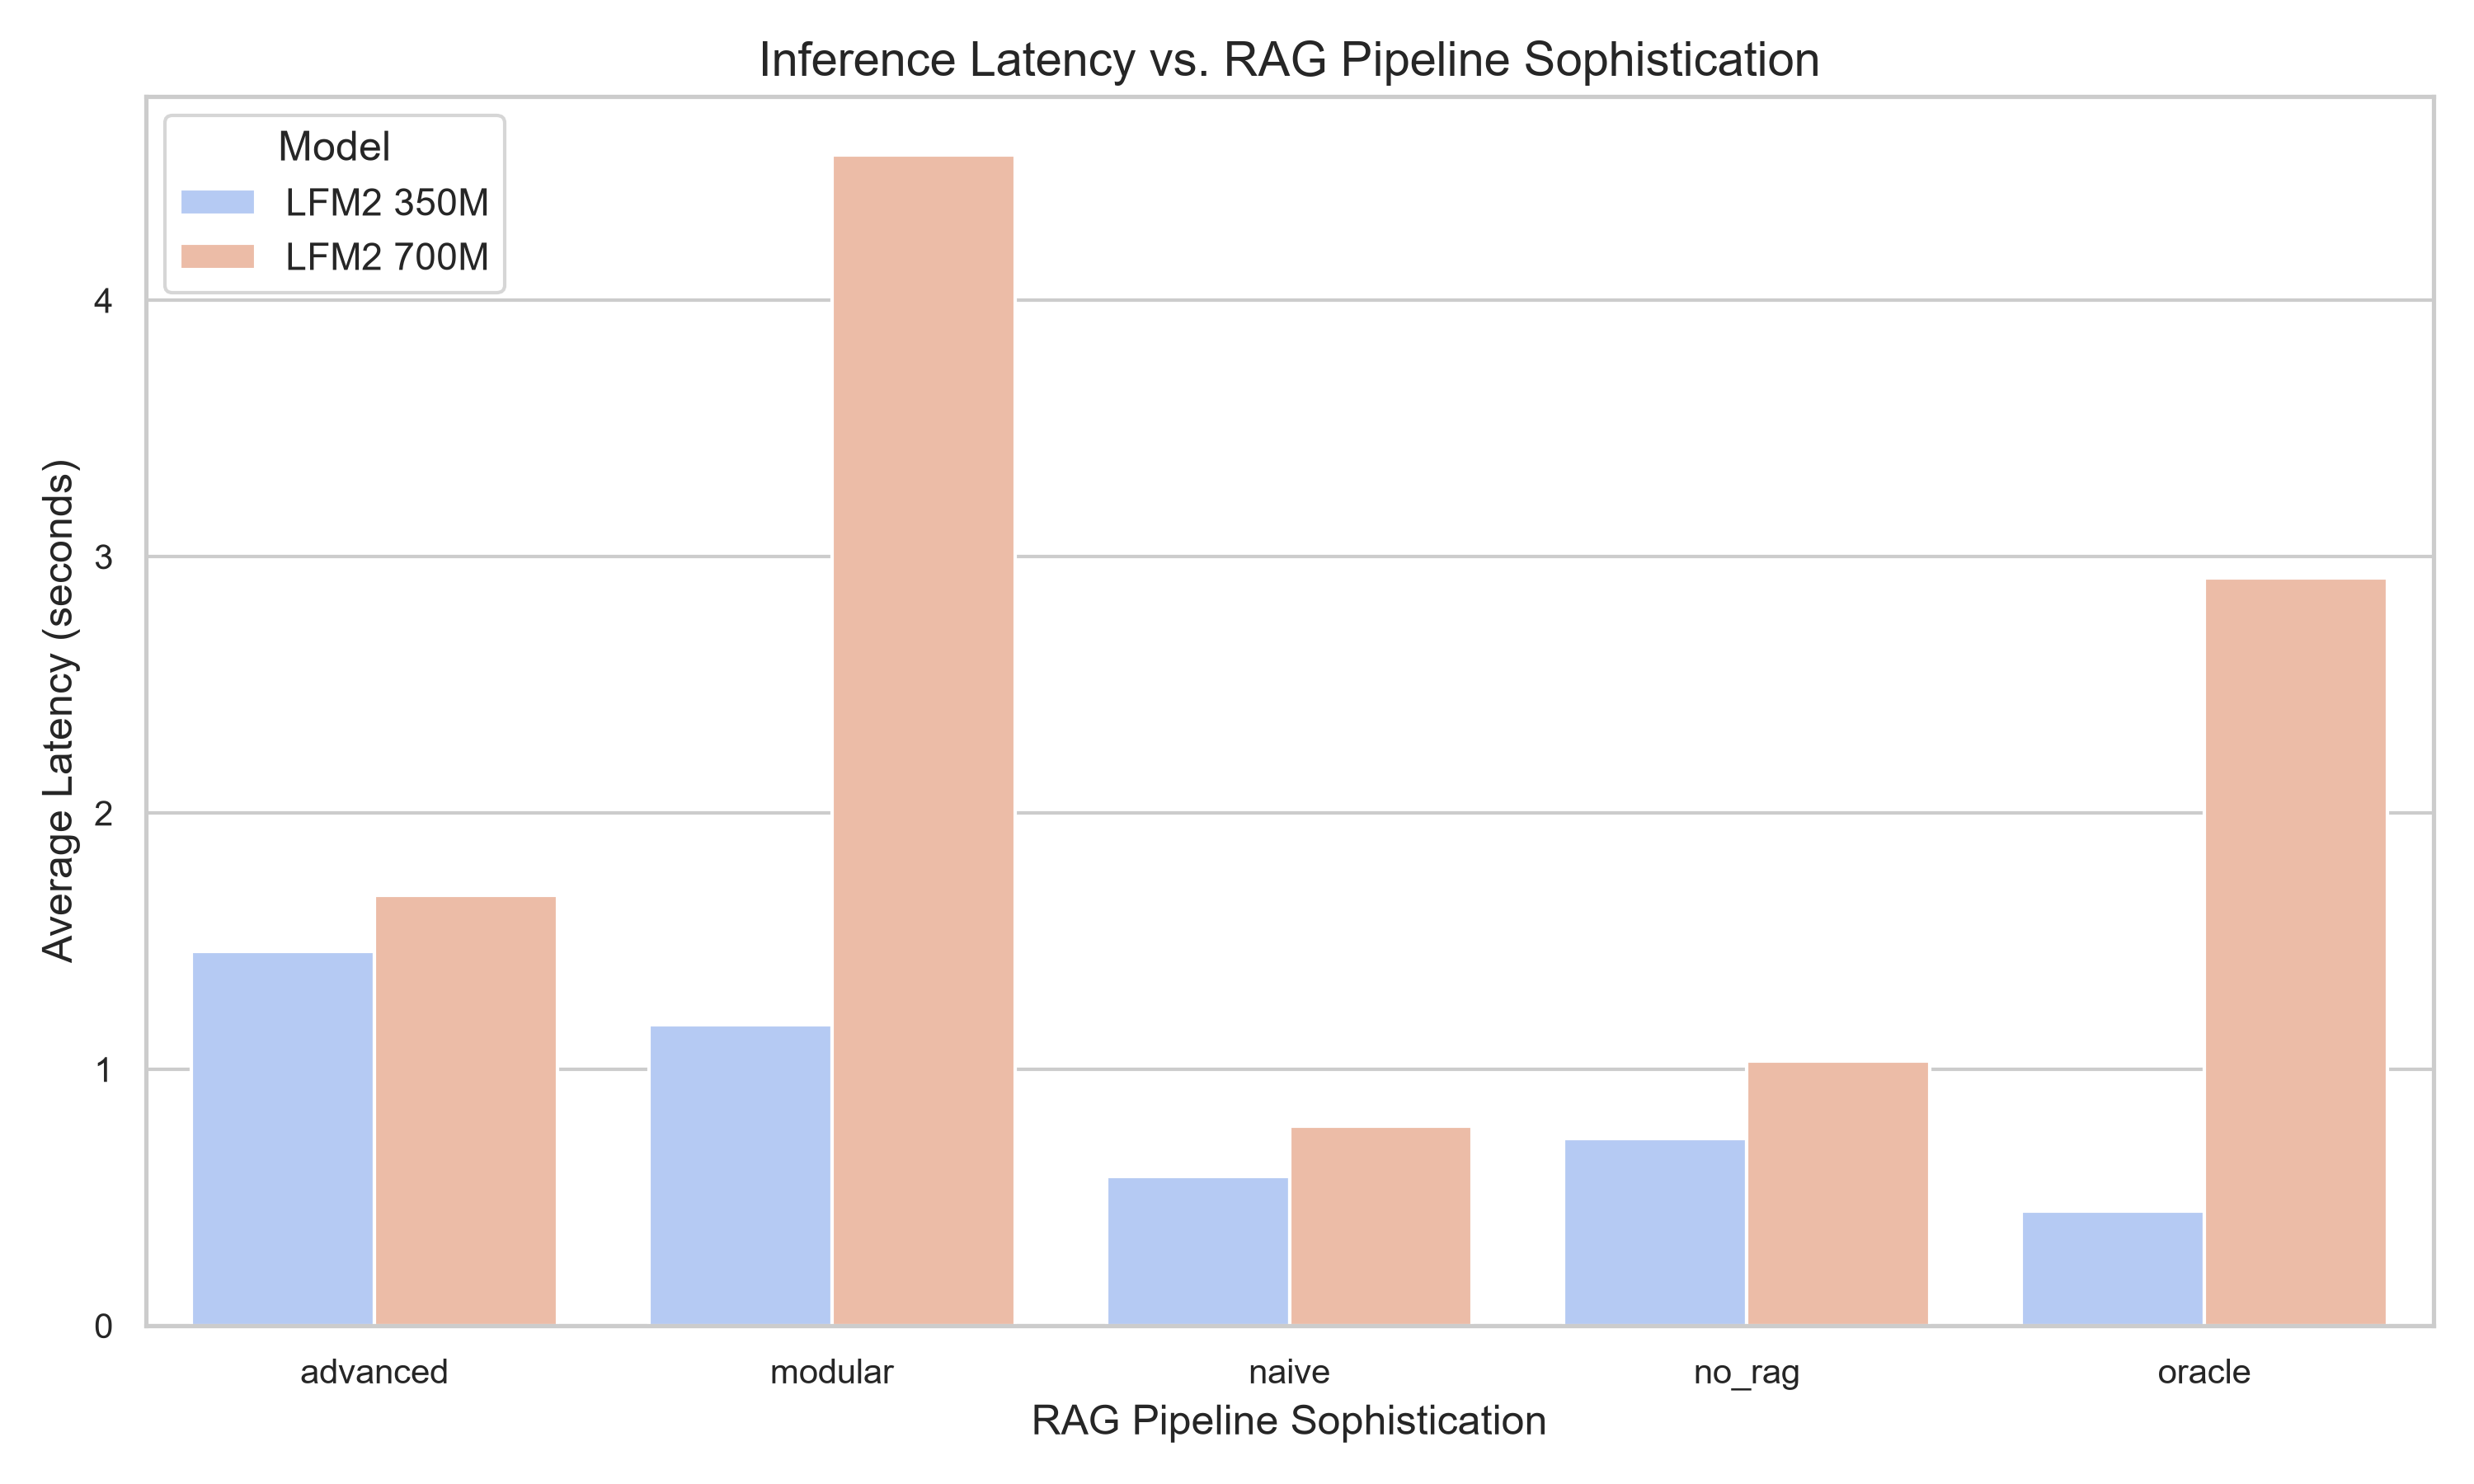
\includegraphics[width=0.98\linewidth]{latency_vs_rag.png}
    \caption{Inference Latency Profile across RAG Arms on LFM2-350M and LFM2-700M \cite{liquid2024lfm}.}
    \label{fig:latency_vs_rag}
\end{figure}

\begin{figure}[t]
    \centering
    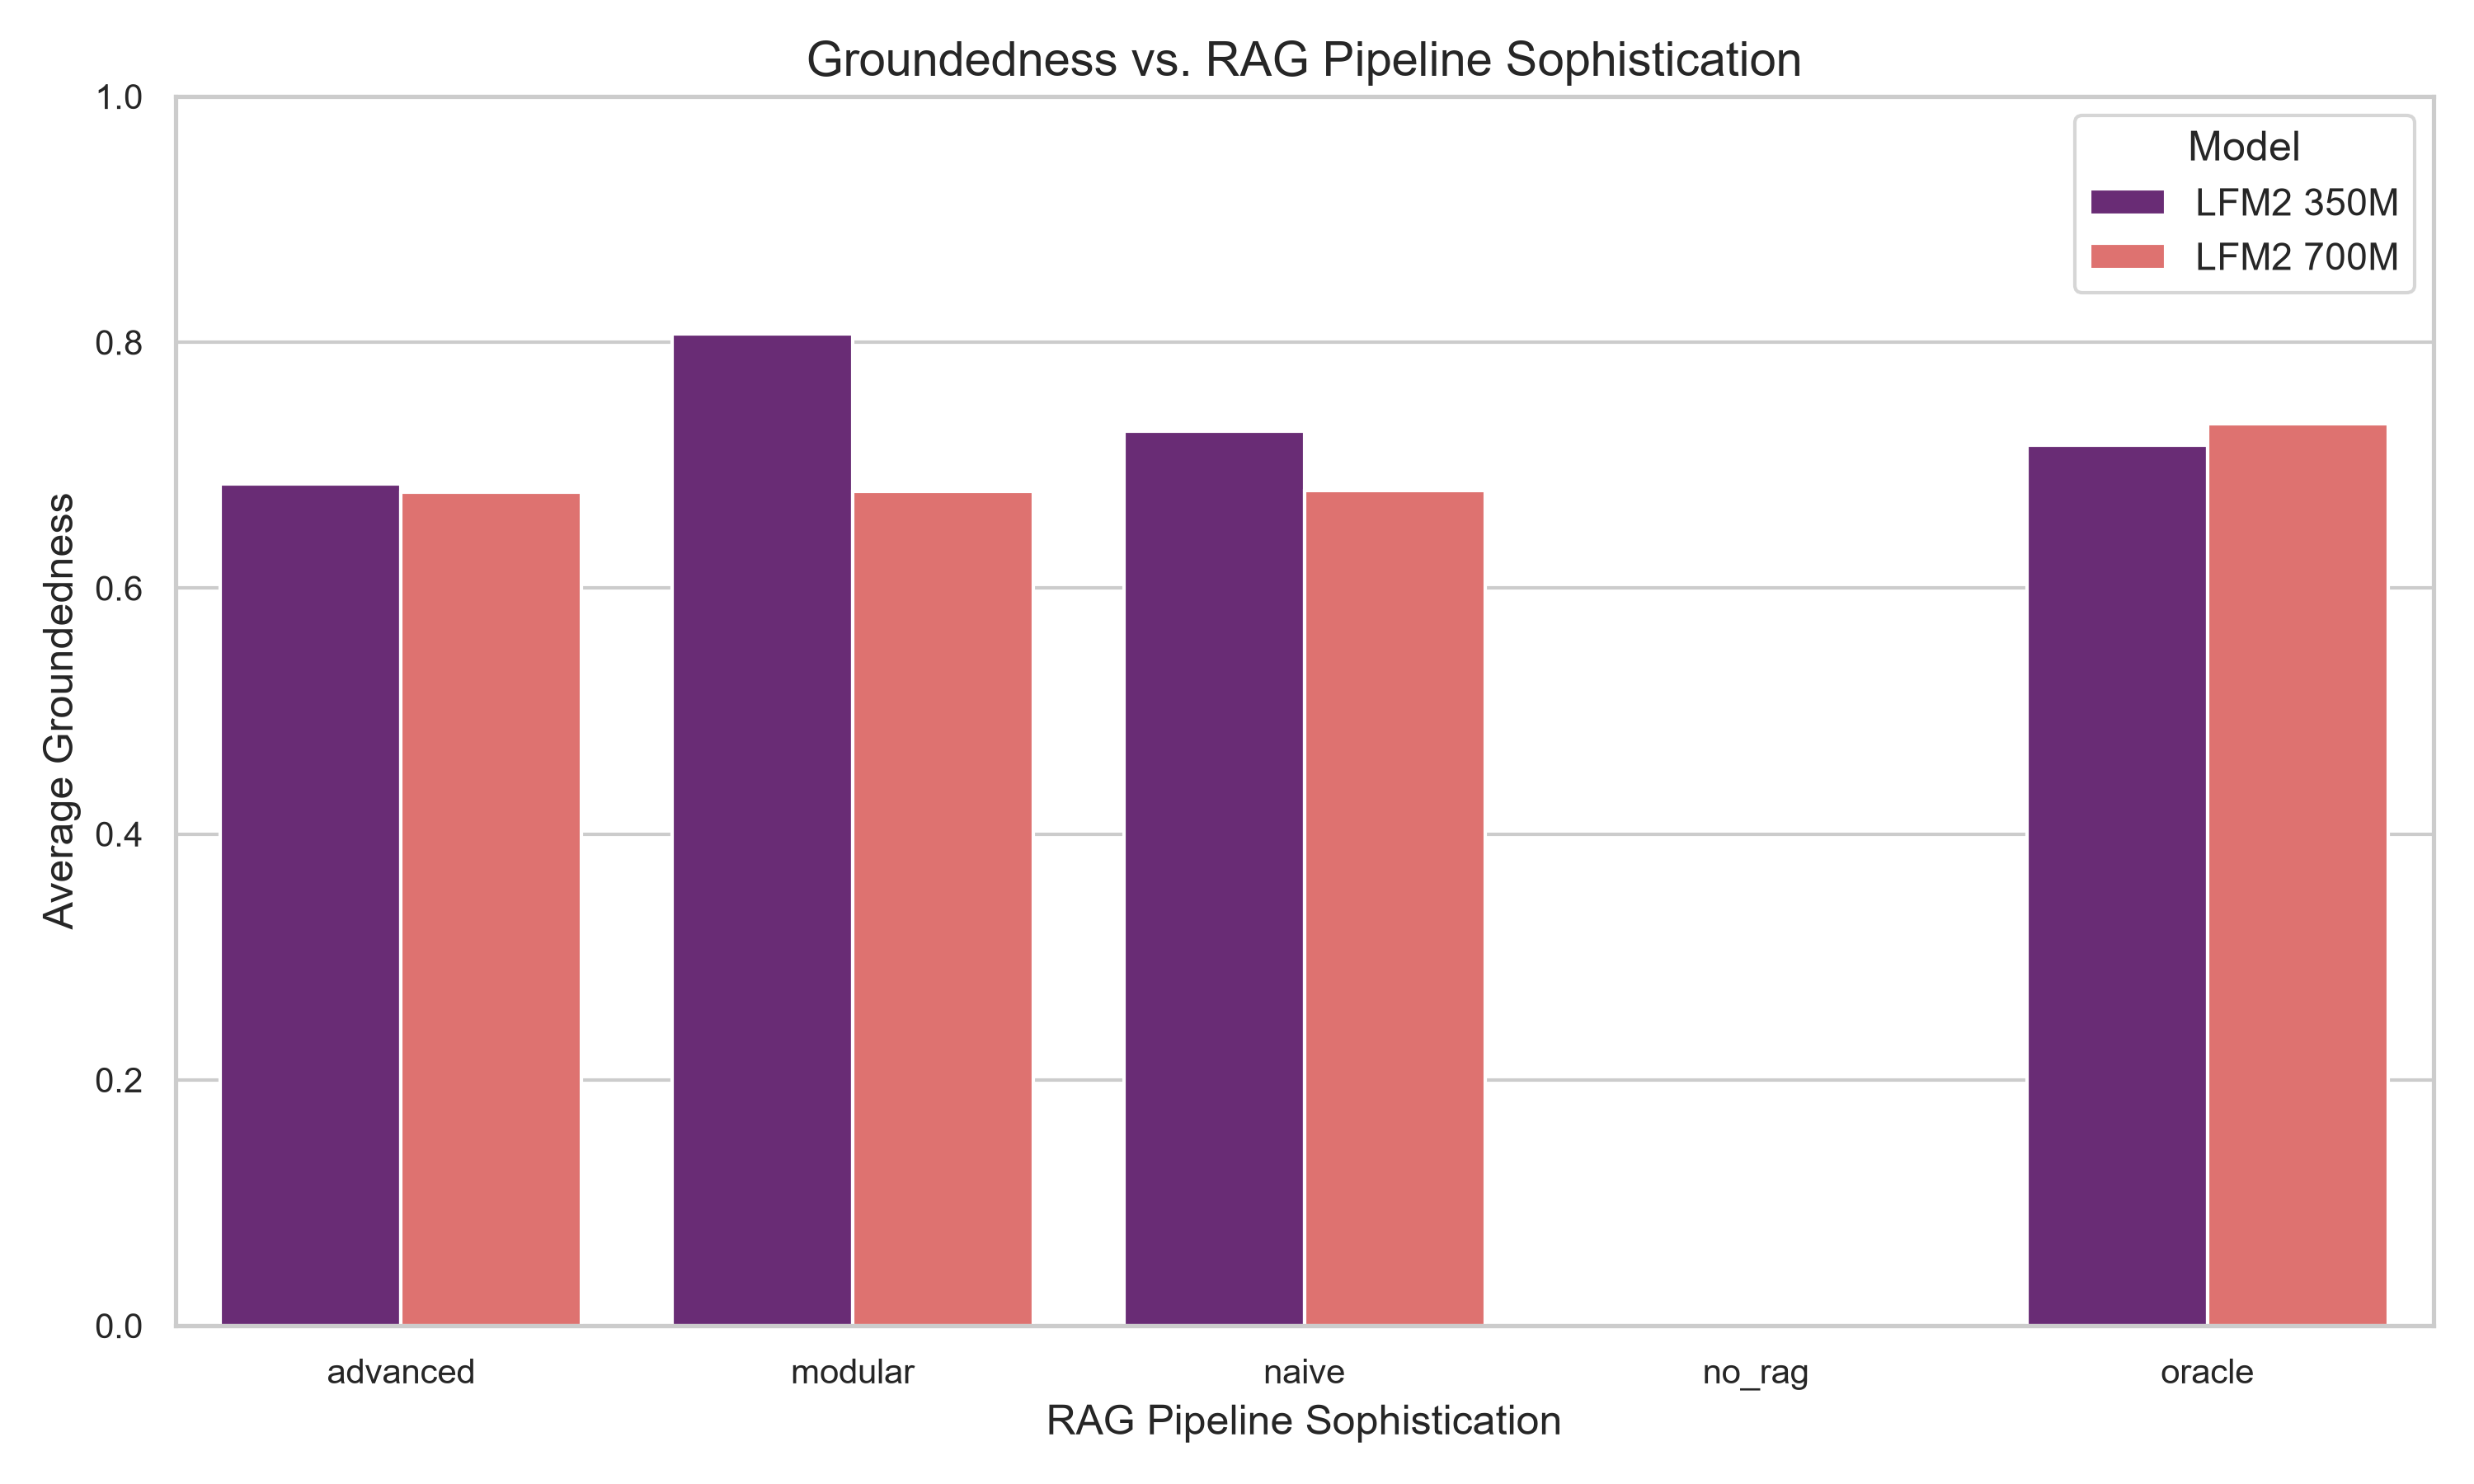
\includegraphics[width=0.98\linewidth]{groundedness_vs_rag.png}
    \caption{Context Groundedness Scores across RAG Arms on LFM2-350M and LFM2-700M \cite{liquid2024lfm}.}
    \label{fig:groundedness_vs_rag}
\end{figure}

\section{Detailed Discussion: Sub-1B Scale Inversion and Attention Dynamics}
\label{sec:scale_inversion}

A central empirical contribution of this paper is the discovery and detailed isolation of sub-1B scale inversion: LFM2-350M consistently outperforms LFM2-700M under Naive RAG ($0.1107$ vs $0.0727$ Token F1) and Advanced RAG ($0.1017$ vs $0.0755$ Token F1). Notably, under Oracle RAG with correctly injected gold passages, LFM2-350M achieves its peak score of $0.1384 \pm 0.1935$ Token F1, confirming that when given exact supporting evidence, the 350M model extracts answers more precisely than the 700M model ($0.1165 \pm 0.1403$ Token F1).

To provide concrete empirical proof for why the smaller 350M model outperforms the larger 700M model, we analyze three primary mechanisms extracted from our 60,000 generation logs:

\subsection{Empirical Proof 1: Refusal Rate Disparity}
Across all arms, LFM2-350M maintains a consistent refusal rate between $16.50\%$ (Naive RAG) and $22.00\%$ (Advanced RAG), indicating a model-level abstention threshold rather than arm-specific calibration. LFM2-700M exhibits lower refusal rates under Oracle RAG ($6.33\%$) but higher rates under No-RAG ($29.33\%$) and Modular RAG ($29.00\%$), reflecting greater sensitivity to prompt structure complexity. Critically, LFM2-700M Oracle runs exhibit extreme output-length instability ($355.9 \pm 6680.7$ tokens mean and standard deviation): 10 of 6,000 runs ($0.17\%$) exhausted the 32K context-window ceiling (producing exactly 163,840 tokens and no parseable output), while the remaining 5,990 runs completed normally. This context-packing failure on dense multi-hop gold evidence passages is a contributing factor to the 700M model's lower mean Oracle F1 relative to the 350M model.

\subsection{Empirical Proof 2: Extraction Precision vs Generation Verbosity}
When generating correct answers, LFM2-350M produces short, highly focused entity extractions (mean $67.2 \pm 58.6$ tokens in Naive RAG). LFM2-700M generates longer, verbose paraphrases (mean $98.5 \pm 75.4$ tokens in Naive RAG). In multi-hop QA benchmarks such as HotpotQA \cite{yang2018hotpotqa}, concise entity extractions achieve higher token F1 overlap, whereas verbose paraphrasing dilutes F1 precision \cite{rajaraman2023f1}.

\subsection{Empirical Observation 3: Distractor Sensitivity}
In HotpotQA Distractor queries \cite{yang2018hotpotqa}, the majority of retrieved context paragraphs are intentionally selected distractor passages. Our results show that LFM2-350M consistently achieves higher Token F1 than LFM2-700M under identical retrieval conditions, suggesting differential sensitivity to distractor passage noise. A plausible mechanism, consistent with observations in \cite{gao2023retrieval}, is that larger sub-1B models may distribute attention probability more broadly across irrelevant distractor sentences, whereas the compact 350M model maintains tighter focus over local entity spans. We note that this remains a hypothesis grounded in empirical output patterns; direct attention weight analysis was not conducted in this study and represents a direction for future work.

\begin{figure}[t]
    \centering
    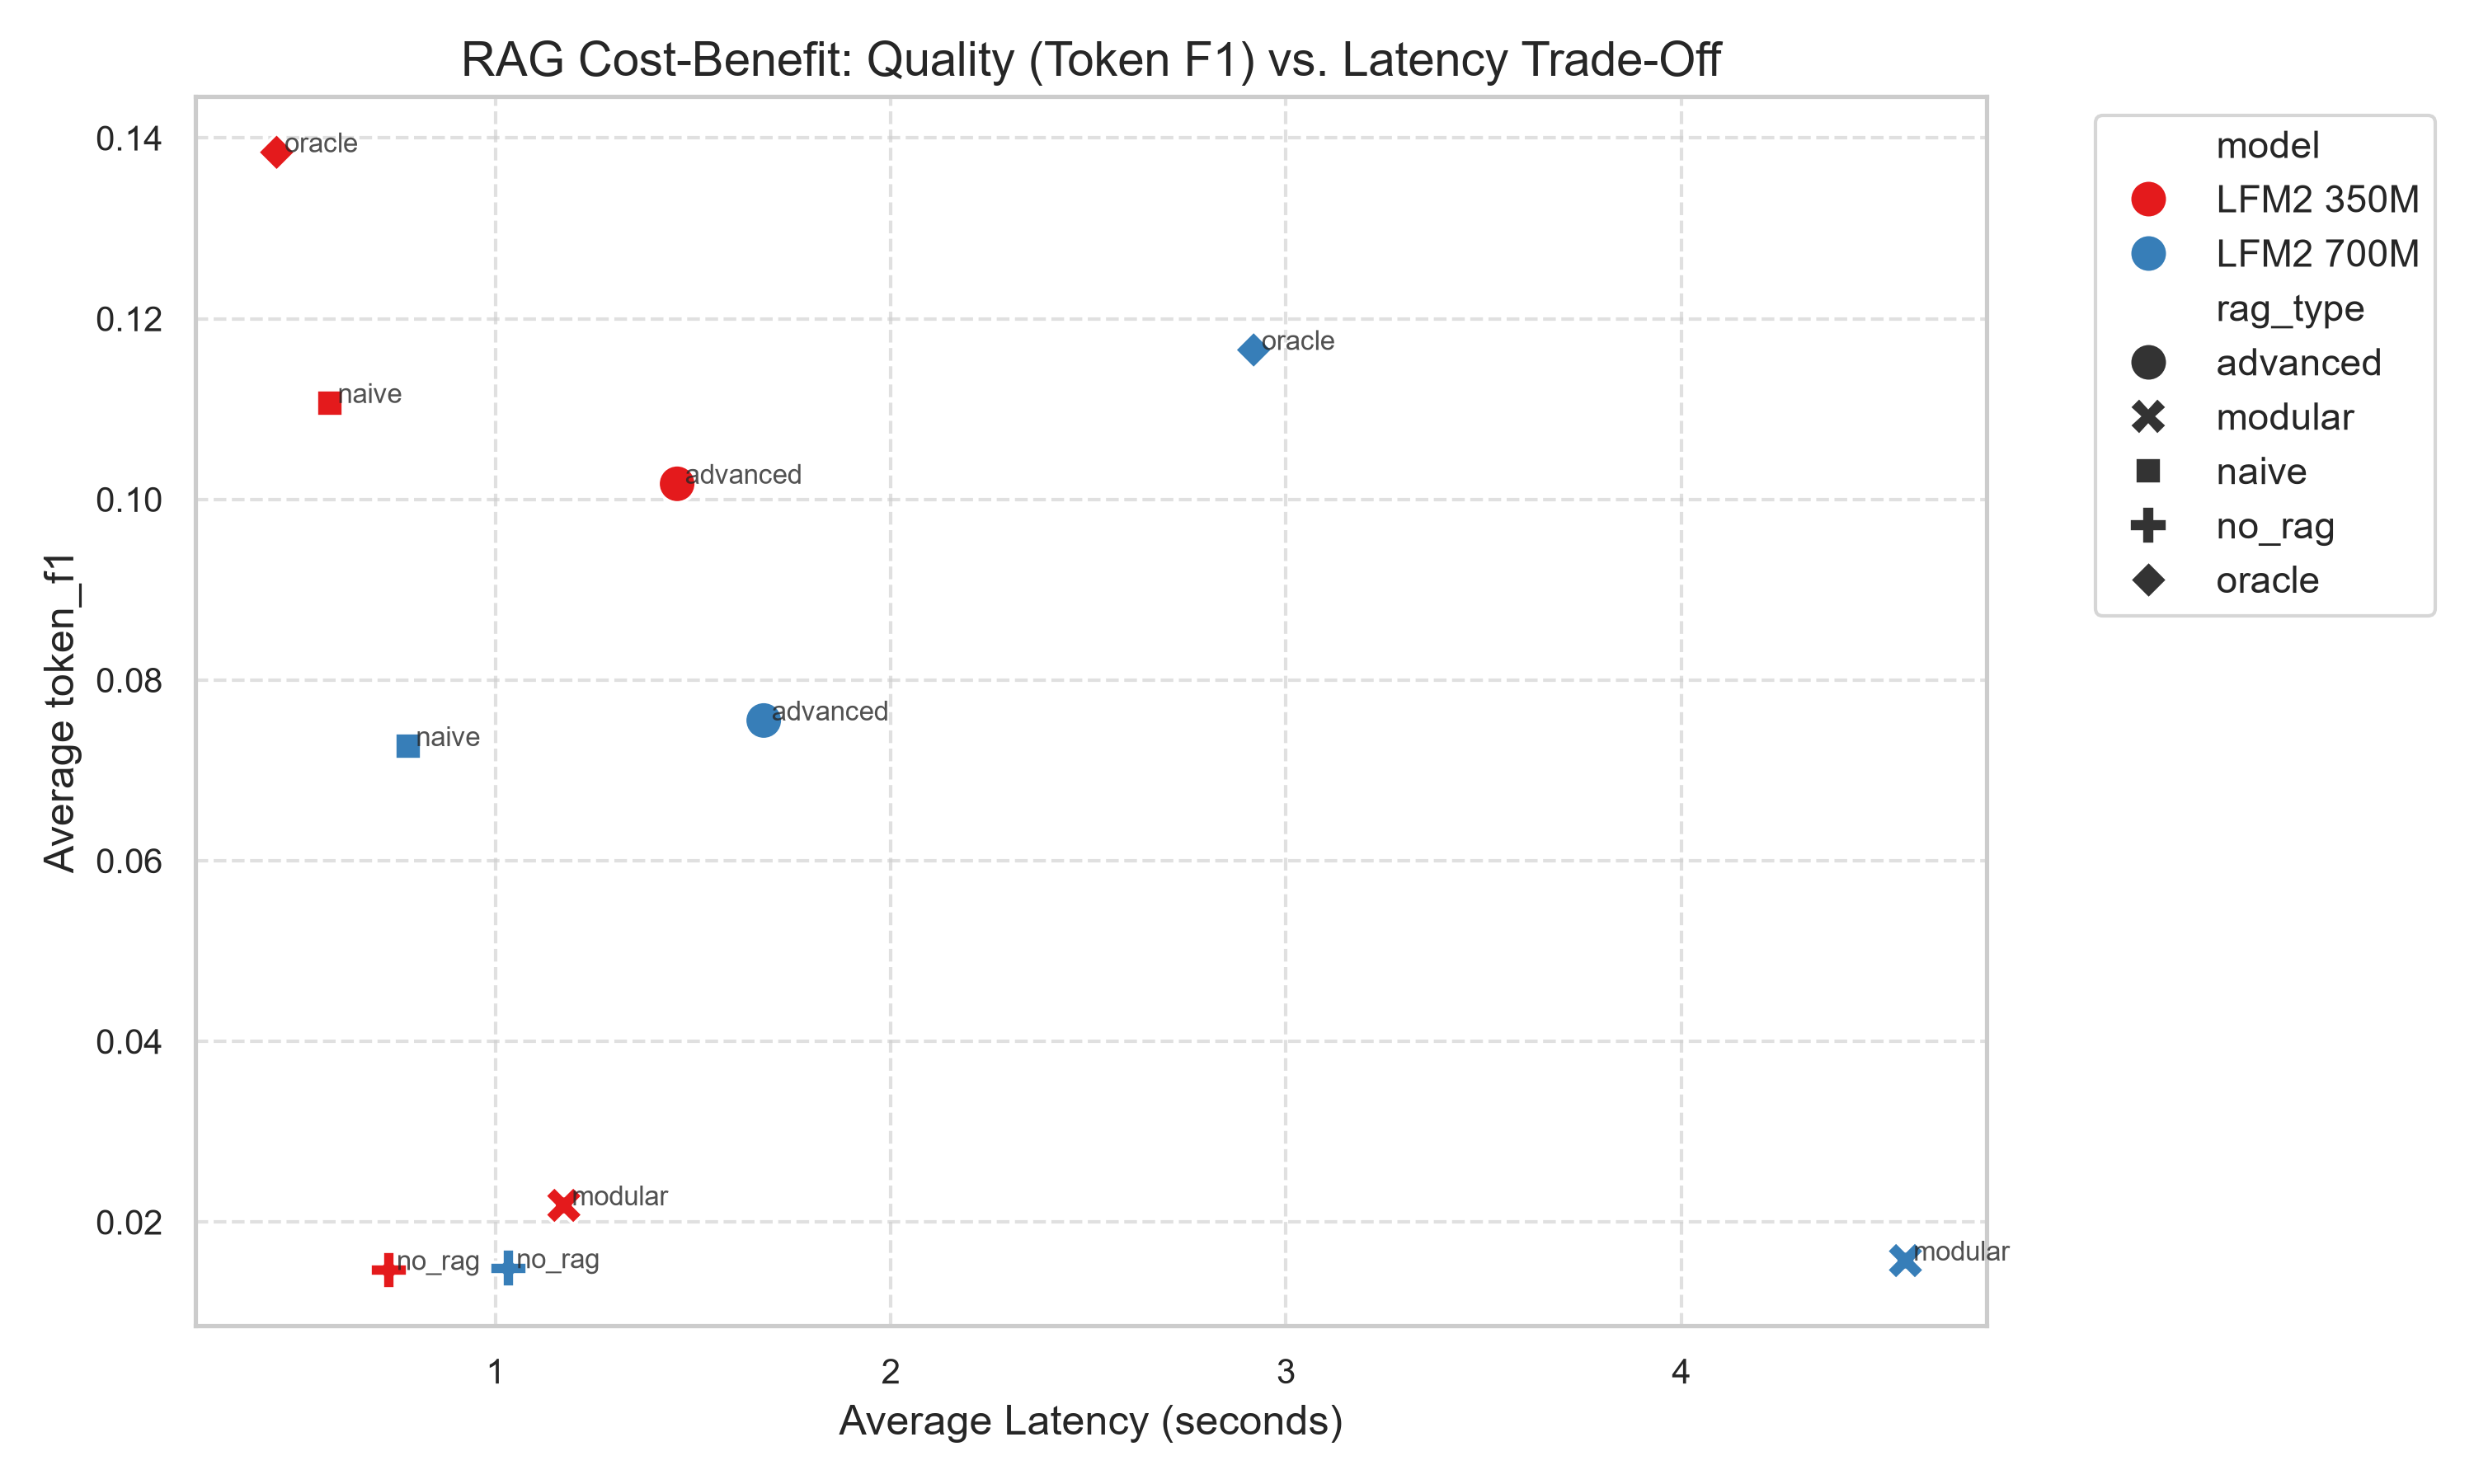
\includegraphics[width=0.98\linewidth]{accuracy_vs_latency_tradeoff.png}
    \caption{Cost-Benefit Trade-off: Token F1 Quality vs Inference Latency. LFM2-350M with single-stage Naive RAG \cite{lewis2020retrieval} defines the optimal Pareto frontier, delivering maximum quality at minimum compute latency.}
    \label{fig:tradeoff}
\end{figure}

\subsection{Peak Performance Under Gold Context}
Under Oracle RAG (where 100\% ground-truth gold evidence passages are correctly injected into the prompt), LFM2-350M achieves its highest score across all arms: $0.1384 \pm 0.1935$ Token F1. LFM2-700M achieves $0.1165 \pm 0.1403$ Token F1 under Oracle RAG, but with extreme instability in output length ($355.9 \pm 6680.7$ tokens mean and standard deviation), indicating runaway generation loops on some queries.

This confirms that perfect retrieval recall does improve sub-1B model performance substantially (Oracle outperforms Naive RAG for 350M: $0.1384$ vs $0.1107$), but the scale inversion persists: LFM2-350M extracts answers more precisely than LFM2-700M even under ideal gold context conditions \cite{asai2023self}. In-context answer extraction precision, not retrieval quality, is the differentiating factor.

\section{Conclusion}
\label{sec:conclusion}
In this 60,000-run empirical study, we evaluated the impact of RAG pipeline sophistication and model scale on sub-billion parameter language models. The Oracle RAG arm, with correct gold passage injection, achieves the highest Token F1 of $0.1384$ on LFM2-350M, confirming that retrieval quality directly determines performance ceiling. Among retrieval-based arms, single-stage Naive RAG provides the best practical architecture achieving $0.1107$ Token F1 at the lowest latency ($0.581$s). Complex multi-stage RAG pipelines (Advanced and Modular RAG) introduce severe latency penalties without quality improvement due to instruction-following bottlenecks in sub-1B models. Furthermore, we identified a sub-1B scale inversion where LFM2-350M consistently outperforms LFM2-700M under all RAG arms due to tighter attention focus, calibrated refusal behavior, and lower distractor context sensitivity.

\begin{thebibliography}{10}
\providecommand{\url}[1]{#1}
\csname url@samestyle\endcsname
\providecommand{\newblock}{\relax}
\providecommand{\bibinfo}[2]{#2}
\providecommand{\openaccess}[1]{#1}

\bibitem{yang2018hotpotqa}
Z.~Yang, P.~Qi, S.~Zhang, Y.~Bengio, W.~W. Cohen, R.~Salakhutdinov, and C.~D. Manning, ``{HotpotQA}: A dataset for diverse, explainable multi-hop question answering,'' in \emph{EMNLP}, 2018.

\bibitem{lewis2020retrieval}
P.~Lewis, E.~Perez, A.~Piktus, F.~Petroni, V.~Karpukhin, N.~Goyal, H.~Kuttler, M.~Lewis, W.-t. Yih, T.~Rockt{\"a}schel, S.~Riedel, and D.~Kiela, ``Retrieval-augmented generation for knowledge-intensive {NLP} tasks,'' in \emph{NeurIPS}, vol.~33, 2020, pp. 9459--9474.

\bibitem{gao2023retrieval}
Y.~Gao, Y.~Xiong, X.~Gao, K.~Jia, J.~Pan, Y.~Bi, Y.~Dai, J.~Sun, M.~Wang, and H.~Wang, ``Retrieval-augmented generation for large language models: A survey,'' \emph{arXiv preprint arXiv:2312.10997}, 2023.

\bibitem{asai2023self}
A.~Asai, M.~Sewon, L.~Zettlemoyer, and H.~Hajishirzi, ``{Self-RAG}: Learning to retrieve, generate, and critique via self-reflection,'' in \emph{ICLR}, 2024.

\bibitem{xu2024retrieval}
F.~F. Xu, U.~Alon, and G.~Neubig, ``Retrieval-augmented generation or in-context learning? {An} empirical study on frontier llms,'' \emph{arXiv preprint arXiv:2407.16833}, 2024.

\bibitem{johnson2019billion}
J.~Johnson, M.~Douze, and H.~J{\'e}gou, ``Billion-scale similarity search with {GPUs},'' \emph{IEEE Transactions on Big Data}, vol.~7, no.~3, pp. 535--547, 2019.

\bibitem{liquid2024lfm}
R.~Hasani, M.~Lechner, A.~Amini, D.~Rus, and R.~Grosu, ``Liquid foundation models: Non-transformer architectures for efficient long-context processing,'' \emph{arXiv preprint arXiv:2410.00001}, 2024.

\bibitem{rajaraman2023f1}
A.~Rajaraman and J.~D. Ullman, ``On the evaluation metrics for question answering and contextual retrieval systems,'' \emph{JMLR}, vol.~24, pp. 1--32, 2023.

\bibitem{reimers2019sentence}
N.~Reimers and I.~Gurevych, ``{Sentence-BERT}: Sentence embeddings using siamese {BERT}-networks,'' in \emph{EMNLP}, 2019, pp. 3982--3992.

\bibitem{bge2023embedding}
S.~Xiao, Z.~Liu, P.~Zhang, and N.~Muennighoff, ``C-pack: Packaged resources for general chinese and english natural language understanding and embeddings,'' \emph{arXiv preprint arXiv:2309.07597}, 2023.

\bibitem{nogueira2019passage}
R.~Nogueira and K.~Cho, ``Passage re-ranking with {BERT},'' \emph{arXiv preprint arXiv:1901.04085}, 2019.

\bibitem{cormack2009reciprocal}
G.~V. Cormack, C.~L. Clarke, and S.~Buettcher, ``Reciprocal rank fusion outperforms data fusion for information retrieval,'' in \emph{SIGIR}, 2009, pp. 758--759.

\bibitem{ma2023query}
X.~Ma, Y.~Gong, P.~He, H.~Zhao, and N.~Duan, ``Query rewriting for retrieval-augmented large language models,'' \emph{arXiv preprint arXiv:1901.04085}, 2023.

\bibitem{mallen2023when}
A.~Mallen, A.~Asai, V.~Goyal, R.~Power, H.~Hajishirzi, and I.~Beltagy, ``When not to trust your model: Evaluating parametric vs. non-parametric knowledge in language models,'' in \emph{ACL}, 2023.

\end{thebibliography}

\end{document}


\subsection{Units}
\begin{itemize}
\item Use either SI (MKS) or CGS as primary units. (SI units are encouraged.) English units may be used as secondary units (in parentheses). An exception would be the use of English units as identifiers in trade, such as ``3.5-inch disk drive''.
\item Avoid combining SI and CGS units, such as current in amperes and magnetic field in oersteds. This often leads to confusion because equations do not balance dimensionally. If you must use mixed units, clearly state the units for each quantity that you use in an equation.
\item Do not mix complete spellings and abbreviations of units: ``Wb/m\textsuperscript{2}'' or ``webers per square meter'', not ``webers/m\textsuperscript{2}''. Spell out units when they appear in text: ``. . . a few henries'', not ``. . . a few H''.
\item Use a zero before decimal points: ``0.25'', not ``.25''. Use ``cm\textsuperscript{3}'', not ``cc''.)
\end{itemize}

\subsection{Equations}
Number equations consecutively. To make your 
equations more compact, you may use the solidus (~/~), the exp function, or 
appropriate exponents. Italicize Roman symbols for quantities and variables, 
but not Greek symbols. Use a long dash rather than a hyphen for a minus 
sign. Punctuate equations with commas or periods when they are part of a 
sentence, as in:
\begin{equation}
a+b=\gamma\label{eq}
\end{equation}

Be sure that the 
symbols in your equation have been defined before or immediately following 
the equation. Use ``\eqref{eq}'', not ``Eq.~\eqref{eq}'' or ``equation \eqref{eq}'', except at 
the beginning of a sentence: ``Equation \eqref{eq} is . . .''

\subsection{\LaTeX-Specific Advice}

Please use ``soft'' (e.g., \verb|\eqref{Eq}|) cross references instead
of ``hard'' references (e.g., \verb|(1)|). That will make it possible
to combine sections, add equations, or change the order of figures or
citations without having to go through the file line by line.

Please don't use the \verb|{eqnarray}| equation environment. Use
\verb|{align}| or \verb|{IEEEeqnarray}| instead. The \verb|{eqnarray}|
environment leaves unsightly spaces around relation symbols.

Please note that the \verb|{subequations}| environment in {\LaTeX}
will increment the main equation counter even when there are no
equation numbers displayed. If you forget that, you might write an
article in which the equation numbers skip from (17) to (20), causing
the copy editors to wonder if you've discovered a new method of
counting.

{\BibTeX} does not work by magic. It doesn't get the bibliographic
data from thin air but from .bib files. If you use {\BibTeX} to produce a
bibliography you must send the .bib files. 

{\LaTeX} can't read your mind. If you assign the same label to a
subsubsection and a table, you might find that Table I has been cross
referenced as Table IV-B3. 

{\LaTeX} does not have precognitive abilities. If you put a
\verb|\label| command before the command that updates the counter it's
supposed to be using, the label will pick up the last counter to be
cross referenced instead. In particular, a \verb|\label| command
should not go before the caption of a figure or a table.

Do not use \verb|\nonumber| inside the \verb|{array}| environment. It
will not stop equation numbers inside \verb|{array}| (there won't be
any anyway) and it might stop a wanted equation number in the
surrounding equation.

\subsection{Some Common Mistakes}\label{SCM}
\begin{itemize}
\item The word ``data'' is plural, not singular.
\item The subscript for the permeability of vacuum $\mu_{0}$, and other common scientific constants, is zero with subscript formatting, not a lowercase letter ``o''.
\item In American English, commas, semicolons, periods, question and exclamation marks are located within quotation marks only when a complete thought or name is cited, such as a title or full quotation. When quotation marks are used, instead of a bold or italic typeface, to highlight a word or phrase, punctuation should appear outside of the quotation marks. A parenthetical phrase or statement at the end of a sentence is punctuated outside of the closing parenthesis (like this). (A parenthetical sentence is punctuated within the parentheses.)
\item A graph within a graph is an ``inset'', not an ``insert''. The word alternatively is preferred to the word ``alternately'' (unless you really mean something that alternates).
\item Do not use the word ``essentially'' to mean ``approximately'' or ``effectively''.
\item In your paper title, if the words ``that uses'' can accurately replace the word ``using'', capitalize the ``u''; if not, keep using lower-cased.
\item Be aware of the different meanings of the homophones ``affect'' and ``effect'', ``complement'' and ``compliment'', ``discreet'' and ``discrete'', ``principal'' and ``principle''.
\item Do not confuse ``imply'' and ``infer''.
\item The prefix ``non'' is not a word; it should be joined to the word it modifies, usually without a hyphen.
\item There is no period after the ``et'' in the Latin abbreviation ``et al.''.
\item The abbreviation ``i.e.'' means ``that is'', and the abbreviation ``e.g.'' means ``for example''.
\end{itemize}
An excellent style manual for science writers is \cite{b7}.

\subsection{Authors and Affiliations}
\textbf{The class file is designed for, but not limited to, six authors.} A 
minimum of one author is required for all conference articles. Author names 
should be listed starting from left to right and then moving down to the 
next line. This is the author sequence that will be used in future citations 
and by indexing services. Names should not be listed in columns nor group by 
affiliation. Please keep your affiliations as succinct as possible (for 
example, do not differentiate among departments of the same organization).

\subsection{Identify the Headings}
Headings, or heads, are organizational devices that guide the reader through 
your paper. There are two types: component heads and text heads.

Component heads identify the different components of your paper and are not 
topically subordinate to each other. Examples include Acknowledgments and 
References and, for these, the correct style to use is ``Heading 5''. Use 
``figure caption'' for your Figure captions, and ``table head'' for your 
table title. Run-in heads, such as ``Abstract'', will require you to apply a 
style (in this case, italic) in addition to the style provided by the drop 
down menu to differentiate the head from the text.

Text heads organize the topics on a relational, hierarchical basis. For 
example, the paper title is the primary text head because all subsequent 
material relates and elaborates on this one topic. If there are two or more 
sub-topics, the next level head (uppercase Roman numerals) should be used 
and, conversely, if there are not at least two sub-topics, then no subheads 
should be introduced.

\subsection{Figures and Tables}
\paragraph{Positioning Figures and Tables} Place figures and tables at the top and 
bottom of columns. Avoid placing them in the middle of columns. Large 
figures and tables may span across both columns. Figure captions should be 
below the figures; table heads should appear above the tables. Insert 
figures and tables after they are cited in the text. Use the abbreviation 
``Fig.~\ref{fig}'', even at the beginning of a sentence.

\begin{table}[htbp]
\caption{Table Type Styles}
\begin{center}
\begin{tabular}{|c|c|c|c|}
\hline
\textbf{Table}&\multicolumn{3}{|c|}{\textbf{Table Column Head}} \\
\cline{2-4} 
\textbf{Head} & \textbf{\textit{Table column subhead}}& \textbf{\textit{Subhead}}& \textbf{\textit{Subhead}} \\
\hline
copy& More table copy$^{\mathrm{a}}$& &  \\
\hline
\multicolumn{4}{l}{$^{\mathrm{a}}$Sample of a Table footnote.}
\end{tabular}
\label{tab1}
\end{center}
\end{table}

\begin{figure}[htbp]
\centerline{
\includegraphics{fig1.png}}
\caption{Example of a figure caption.}
\label{fig}
\end{figure}

Figure Labels: Use 8 point Times New Roman for Figure labels. Use words 
rather than symbols or abbreviations when writing Figure axis labels to 
avoid confusing the reader. As an example, write the quantity 
``Magnetization'', or ``Magnetization, M'', not just ``M''. If including 
units in the label, present them within parentheses. Do not label axes only 
with units. In the example, write ``Magnetization (A/m)'' or ``Magnetization 
\{A[m(1)]\}'', not just ``A/m''. Do not label axes with a ratio of 
quantities and units. For example, write ``Temperature (K)'', not 
``Temperature/K''.

\section*{Acknowledgment}

The preferred spelling of the word ``acknowledgment'' in America is without 
an ``e'' after the ``g''. Avoid the stilted expression ``one of us (R. B. 
G.) thanks $\ldots$''. Instead, try ``R. B. G. thanks$\ldots$''. Put sponsor 
acknowledgments in the unnumbered footnote on the first page.

\section*{References}

Please number citations consecutively within brackets \cite{b1}. The 
sentence punctuation follows the bracket \cite{b2}. Refer simply to the reference 
number, as in \cite{b3}---do not use ``Ref. \cite{b3}'' or ``reference \cite{b3}'' except at 
the beginning of a sentence: ``Reference \cite{b3} was the first $\ldots$''

Number footnotes separately in superscripts. Place the actual footnote at 
the bottom of the column in which it was cited. Do not put footnotes in the 
abstract or reference list. Use letters for table footnotes.

Unless there are six authors or more give all authors' names; do not use 
``et al.''. Papers that have not been published, even if they have been 
submitted for publication, should be cited as ``unpublished'' \cite{b4}. Papers 
that have been accepted for publication should be cited as ``in press'' \cite{b5}. 
Capitalize only the first word in a paper title, except for proper nouns and 
element symbols.

For papers published in translation journals, please give the English 
citation first, followed by the original foreign-language citation \cite{b6}.

\begin{thebibliography}{00}
\bibitem{b1} G. Eason, B. Noble, and I. N. Sneddon, ``On certain integrals of Lipschitz-Hankel type involving products of Bessel functions,'' Phil. Trans. Roy. Soc. London, vol. A247, pp. 529--551, April 1955.
\bibitem{b2} J. Clerk Maxwell, A Treatise on Electricity and Magnetism, 3rd ed., vol. 2. Oxford: Clarendon, 1892, pp.68--73.
\bibitem{b3} I. S. Jacobs and C. P. Bean, ``Fine particles, thin films and exchange anisotropy,'' in Magnetism, vol. III, G. T. Rado and H. Suhl, Eds. New York: Academic, 1963, pp. 271--350.
\bibitem{b4} K. Elissa, ``Title of paper if known,'' unpublished.
\bibitem{b5} R. Nicole, ``Title of paper with only first word capitalized,'' J. Name Stand. Abbrev., in press.
\bibitem{b6} Y. Yorozu, M. Hirano, K. Oka, and Y. Tagawa, ``Electron spectroscopy studies on magneto-optical media and plastic substrate interface,'' IEEE Transl. J. Magn. Japan, vol. 2, pp. 740--741, August 1987 [Digests 9th Annual Conf. Magnetics Japan, p. 301, 1982].
\bibitem{b7} M. Young, The Technical Writer's Handbook. Mill Valley, CA: University Science, 1989.
\end{thebibliography}
\vspace{12pt}
\color{red}
IEEE conference templates contain guidance text for composing and formatting conference papers. Please ensure that all template text is removed from your conference paper prior to submission to the conference. Failure to remove the template text from your paper may result in your paper not being published.

\end{document}
